\documentclass{article}
\usepackage{graphicx}

\begin{document}
\title{\Large Assignment 7}
\author{Jianqiang Du\\\\017547307}
\maketitle

\section{Exercise 14.14: a, b, and c.}
\begin{itemize}
\item[a.]Which of the following are asserted by the network \textit{structure}?
	\begin{itemize}
	\item[(i)]\textbf P(\textit B,\textit I,\textit M) = \textbf P(\textit B)\textbf P(\textit I)\textbf P(\textit M).
	\item[(ii)]\textbf P(\textit J$\vert$\textit G) = \textbf P(\textit J$\vert$\textit G,\textit I).
	\item[(iii)]\textbf P(\textit M$\vert$\textit G,\textit B,\textit I) = \textbf P(\textit M$\vert$\textit G,\textit B,\textit I,\textit J).
	\begin{figure}[h!]
	\centering
	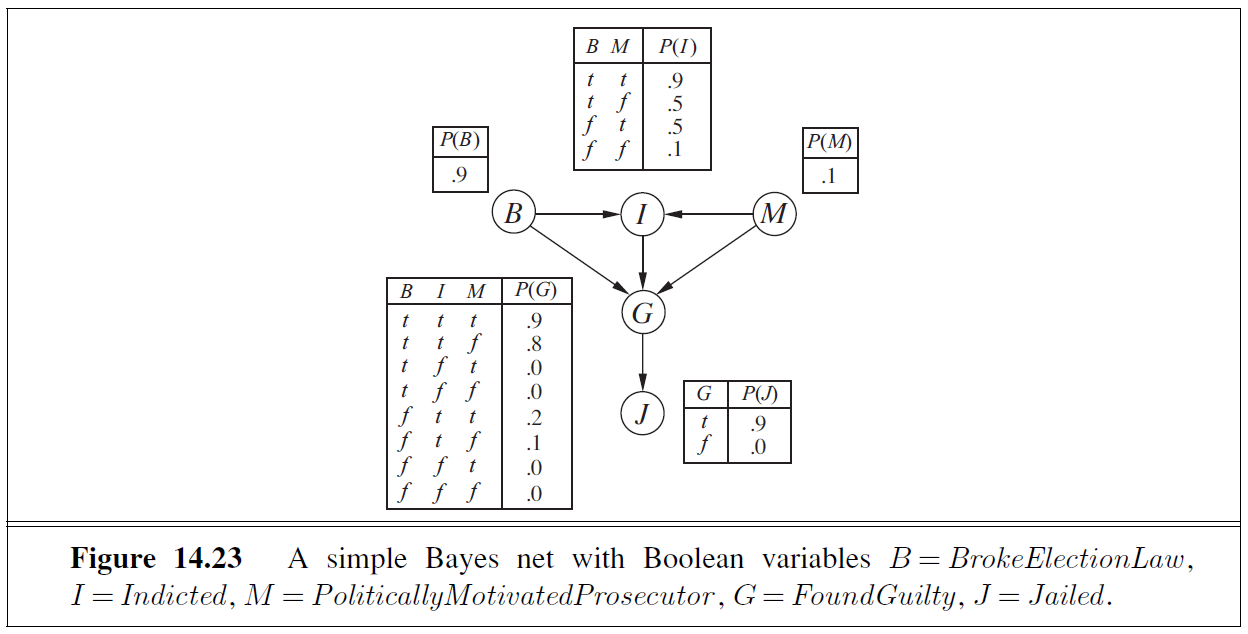
\includegraphics[width=0.8\textwidth]{figure_14_23.png}
	\end{figure}
	\item[\textbf{Answer:}]ii, iii
	\end{itemize}
\item[b.]Calculate the value of \textit P(\textit b,\textit i,$\neg$\textit m,\textit g,\textit j).
	\begin{itemize}
	\item[\textbf{Answer:}]\textit P(\textit b,\textit i,$\neg$\textit m,\textit g,\textit j) = P(b)P(i$\vert$b,$\neg$m)P($\neg$m)P(g$\vert$b,i,$\neg$m)P(j$\vert$g) = 0.9*0.5*0.9*0.8*0.9=0.2916
	\end{itemize}
\item[c.]Calculate the probability that someone goes to jail given that they broke the law, have been indicted, and face a politically motivated prosecutor.
	\begin{itemize}
	\item[\textbf{Answer:}]P(j$\vert$b,i,m)=$\frac{\sum_{g^{'}}P(j,b,i,m,g^{'})}{\sum_{j^{'},g^{'}}P(j^{'},b,i,m,g^{'})}$\\=$\frac{\sum_{g^{'}}P(j\vert g^{'})P(b)P(i\vert b,m)P(m)P(g^{'}\vert b,i,m)}{\sum_{j^{'},g^{'}}P(j^{'}\vert g^{'})P(b)P(i\vert b,m)P(m)P(g^{'}\vert b,i,m)}$\\=$\frac{P(b)P(i\vert b,m)P(m)\sum_{g^{'}}P(j\vert g^{'})P(g^{'}\vert b,i,m)}{P(b)P(i\vert b,m)P(m)\sum_{j^{'},g^{'}}P(j^{'}\vert g^{'})P(g^{'}\vert b,i,m)}$\\=$\frac{P(j\vert g)P(g\vert b,i,m)+P(j\vert\neg g)P(\neg g\vert b,i,m)}{P(j\vert g)P(g\vert b,i,m)+P(j\vert\neg g)P(\neg g\vert b,i,m)+P(\neg j\vert g)P(g\vert b,i,m)+P(\neg j\vert\neg g)P(\neg g\vert b,i,m)}$\\=$\frac{0.9*0.9+0}{0.9*0.9+0+0.1*0.9+1*0.1}$\\=$\frac{0.81}{0.81+0.09+0.1}$\\=$\frac{0.81}{1}$\\=0.81
	\end{itemize}
\end{itemize}

\section{}In Figure 1, suppose we observe an unending sequence of days on which the umbrella appears. As the days go by, the probability of rain on the current day increases toward a fixed point, we expect that $\vec{\textit P}(\textit R_{t}\vert \textit u_{1:t}) = \vec{\textit P}$($\textit R_{t-1}\vert\textit u_{1:t-1}) = \langle\rho, 1 - \rho\rangle$. Find $\rho$.
	\begin{figure}[h!]
	\centering
	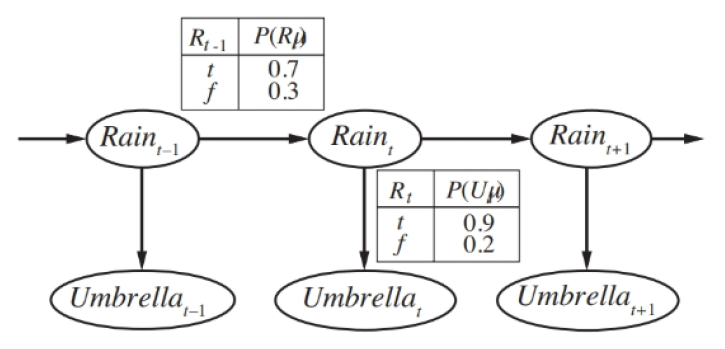
\includegraphics[width=0.8\textwidth]{figure_1.png}
	\caption{Bayesian network structure and conditional distributions describing the umbrella world. The transition model is $\vec{\textit P}(\textit R\vert\textit R_{t-1})$ and the sensor model is $\vec{\textit P}(\textit U\vert\textit R_{t})$.}
	\end{figure}
	\begin{itemize}
	\item[\textbf{Answer:}]$\vec{P}(R_{t}\vert u_{1:t})=\alpha\vec{P}(u_{t}\vert R_{t})\sum_{R_{t-1}}\vec{P}(R_{t}\vert R_{t-1})\vec{P}(R_{t-1}\vert u_{1:t-1})$\\=$\alpha\vec{P}(u_{t}\vert R_{t})(\langle P(R_{t}\vert R_{t-1})P(R_{t-1}\vert u_{1:t-1}),P(\neg R_{t}\vert R_{t-1})P(R_{t-1}\vert u_{1:t-1})\rangle+\\\langle P(R_{t}\vert\neg R_{t-1})P(\neg R_{t-1}\vert u_{1:t-1}),P(\neg R_{t}\vert\neg R_{t-1})P(\neg R_{t-1}\vert u_{1:t-1})\rangle)$\\=$\alpha\langle0.9,0.2\rangle(\langle0.7*\rho,0.3*\rho\rangle+\langle0.3*(1-\rho),0.7*(1-\rho)\rangle)$\\=$\alpha\langle0.27+0.36\rho,0.14-0.08\rho\rangle$=$\langle\rho,1-\rho\rangle$\\$\alpha=\frac{1}{0.27+0.36\rho+0.14-0.08\rho}$=$\frac{1}{0.41+0.28\rho}$\\$\rho=\frac{0.27+0.36\rho}{0.41+0.28\rho}$\\$\rho(0.41+0.28\rho)=0.27+0.36\rho$\\$28\rho^2+5\rho-27=0$\\$\rho=\frac{-5\pm\sqrt{25+4*28*27}}{56}$=0.8967 or -1.0753\\$\rho$=0.8967
	\end{itemize}

\section{}A professor wants to know if students are getting enough sleep. Each day, the professor observes whether the students sleep in class, and whether they have red eyes. The professor has the following domain theory:
	\begin{itemize}
	\item The prior probability of getting enough sleep, with no observations, is 0.7.
	\item The probability of getting enough sleep on night t is 0.8 given that the student got enough sleep the previous night, and 0.3 if not.
	\item The probability of having red eyes is 0.2 if the student got enough sleep, and 0.7 if not.
	\item The probability of sleeping in class is 0.1 if the student got enough sleep, and 0.3 if not.
	\item[(a)]Formulate this information as a hidden Markov model that has only a single observation variable. Give a bayesian network and conditional distributions.
	\item[\textbf{Answer:}]as below
		\begin{figure}[h!]
		\centering
		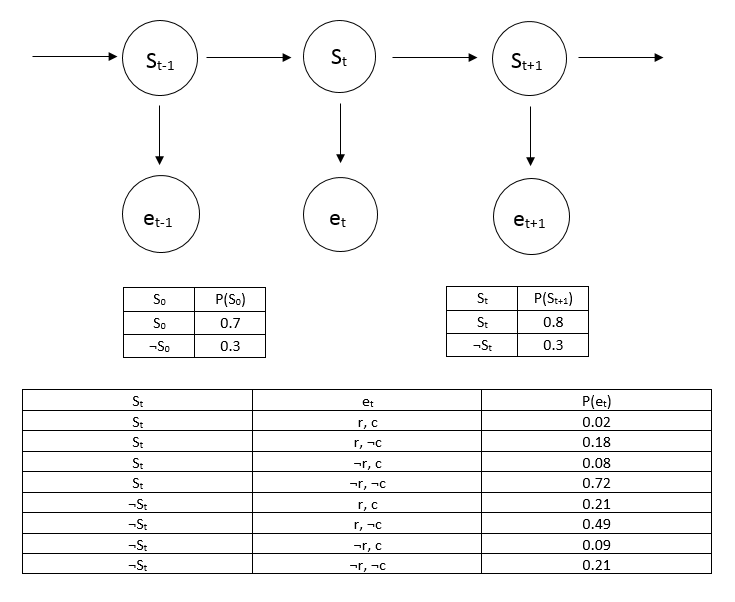
\includegraphics[width=1\textwidth]{hmm.png}
		\end{figure}
	\item[(b)]Consider the following evidences, and compute $\vec{\textit P}(ES_{2}\vert\vec{\textit e}_{1:2})$ and $\vec{\textit P}(ES_{1}\vert\vec{\textit e}_{1:3})$.
		\begin{itemize}
		\item[$\bullet$]$\vec{\textit e}_{1}$ = not red eyes, not sleeping in class
		\item[$\bullet$]$\vec{\textit e}_{2}$ = red eyes, not sleeping in class
		\item[$\bullet$]$\vec{\textit e}_{3}$ = red eyes, sleeping in class
		\end{itemize}
	\item[\textbf{Answer:}]$\vec P(ES_1\vert\vec e_1)=\alpha\vec P(\vec e_1\vert ES_1)\sum_{ES_0}{\vec P(ES_1\vert ES_0)P(ES_0\vert\vec e_0)}$\\=$\alpha\vec P(\vec e_1\vert ES_1)(\langle P(ES_1\vert ES_0)P(ES_0\vert \vec e_0),P(\neg ES_1\vert ES_0)P(ES_0\vert\vec e_0)\rangle+\\\langle P(ES_1\vert\neg ES_0)P(\neg ES_0\vert\vec e_0),P(\neg ES_1\vert\neg ES_0)P(\neg ES_0\vert\vec e_0)\rangle$\\=$\alpha\langle0.72,0.21\rangle(\langle0.8,0.2\rangle*0.7+\langle0.3,0.7\rangle*0.3)$\\=$\alpha\langle0.468,0.0735\rangle$\\=$\langle\frac{0.468}{0.468+0.0735},\frac{0.0735}{0.468+0.0735}\rangle$\\=$\langle0.8643,0.1357\rangle$\\$\vec P(ES_2\vert\vec e_{1:2})=\alpha\vec P(\vec e_1\vert ES_1)\sum_{ES_1}\vec P(ES_2\vert ES_1)P(ES_1\vert\vec e_1)$\\=$\alpha\langle0.18,0.49\rangle(\langle0.8,0.2\rangle*0.8643+\langle0.3,0.7\rangle*0.1357)$\\=$\alpha\langle0.18,0.49\rangle\langle0.73215,0.26785\rangle$\\=$\alpha\langle0.131787,0.131247\rangle$\\=$\langle\frac{0.131787}{0.263034},\frac{0.131247}{0.263034}\rangle$\\=$\langle0.5010,0.4990\rangle$\\$\vec P(ES_1\vert\vec e_{1:3})=\alpha\vec P(ES_1\vert\vec e_1)\sum_{ES_2}P(\vec e_2\vert ES_2)P(\vec e_3\vert ES_2)\vec P(ES_2\vert ES_1)$\\=$\alpha\vec P(ES_1\vert\vec e_1)P(\vec e_3)\sum_{ES_2}P(\vec e_2\vert ES_2)\vec P(ES_2\vert ES_1)$\\=$\alpha\vec P(ES_1\vert\vec e_1)P(\vec e_3)(\langle P(\vec e_2\vert ES_2)P(ES_2\vert ES_1),P(\vec e_2\vert ES_2)P(ES_2\vert\neg ES_1)\rangle+\langle P(\vec e_2\vert\neg ES_2)P(\neg ES_2\vert ES_1),P(\vec e_2\vert\neg ES_2)P(\neg ES_2\vert\neg ES_1)\rangle)$\\=$\beta\langle0.8643,0.1357\rangle(\langle0.8,0.3\rangle*0.18+\langle0.2,0.7\rangle*0.49)$\\=$\beta\langle0.8643,0.1357\rangle\langle0.242,0.397\rangle$\\=$\beta\langle0.2091606,0.0538729\rangle$\\=$\langle\frac{0.2091606}{0.2630335},\frac{0.0538729}{0.2630335}\rangle$\\=$\langle0.7952,0.2048\rangle$
	\end{itemize}
\end{document}